
\documentclass[useAMS,usenatbib,article]{mn2e}

\usepackage{longtable}
\usepackage[]{graphicx}
\usepackage{amsmath}
\usepackage{natbib}
\bibliographystyle{mn2e}
%\usepackage{tabularx}
%\usepackage{bm}
%\usepackage{color}
%\usepackage{hyperref}

%% Sometimes a paper's abstract is too long to fit on the
%% title page in preprint2 mode. When that is the case,
%% use the longabstract style option.

%% \documentclass[preprint2,longabstract]{aastex}
\newcommand\aj{{AJ}}%
\newcommand\actaa{{Acta Astron.}}%
\newcommand\araa{{ARA\&A}}%
\newcommand\apj{{ApJ}}%
\newcommand\apjl{{ApJ}}%
\newcommand\apjs{{ApJS}}%
\newcommand\ao{{Appl.~Opt.}}%
\newcommand\apss{{Ap\&SS}}%
\newcommand\aap{{A\&A}}%
\newcommand\aapr{{A\&A~Rev.}}%
\newcommand\aaps{{A\&AS}}%
\newcommand\azh{{AZh}}%
\newcommand\baas{{BAAS}}%
\newcommand\caa{{Chinese Astron. Astrophys.}}%
\newcommand\cjaa{{Chinese J. Astron. Astrophys.}}%
\newcommand\icarus{{Icarus}}%
\newcommand\jcap{{J. Cosmology Astropart. Phys.}}%
\newcommand\jrasc{{JRASC}}%
\newcommand\memras{{MmRAS}}%
\newcommand\mnras{{MNRAS}}%
\newcommand\na{{New A}}%
\newcommand\nar{{New A Rev.}}%
\newcommand\pra{{Phys.~Rev.~A}}%
\newcommand\prb{{Phys.~Rev.~B}}%
\newcommand\prc{{Phys.~Rev.~C}}%
\newcommand\prd{{Phys.~Rev.~D}}%
\newcommand\pre{{Phys.~Rev.~E}}%
\newcommand\prl{{Phys.~Rev.~Lett.}}%
\newcommand\pasa{{PASA}}%
\newcommand\pasp{{PASP}}%
\newcommand\pasj{{PASJ}}%
\newcommand\qjras{{QJRAS}}%
\newcommand\rmxaa{{Rev. Mexicana Astron. Astrofis.}}%
\newcommand\skytel{{S\&T}}%
\newcommand\solphys{{Sol.~Phys.}}%
\newcommand\sovast{{Soviet~Ast.}}%
\newcommand\ssr{{Space~Sci.~Rev.}}%
\newcommand\zap{{ZAp}}%
\newcommand\nat{{Nature}}%
\newcommand\iaucirc{{IAU~Circ.}}%
\newcommand\aplett{{Astrophys.~Lett.}}%
\newcommand\apspr{{Astrophys.~Space~Phys.~Res.}}%
\newcommand\bain{{Bull.~Astron.~Inst.~Netherlands}}%
\newcommand\fcp{{Fund.~Cosmic~Phys.}}%
\newcommand\gca{{Geochim.~Cosmochim.~Acta}}%
\newcommand\grl{{Geophys.~Res.~Lett.}}%
\newcommand\jcp{{J.~Chem.~Phys.}}%
\newcommand\jgr{{J.~Geophys.~Res.}}%
\newcommand\jqsrt{{J.~Quant.~Spec.~Radiat.~Transf.}}%
\newcommand\memsai{{Mem.~Soc.~Astron.~Italiana}}%
\newcommand\nphysa{{Nucl.~Phys.~A}}%
\newcommand\physrep{{Phys.~Rep.}}%
\newcommand\physscr{{Phys.~Scr}}%
\newcommand\planss{{Planet.~Space~Sci.}}%
\newcommand\procspie{{Proc.~SPIE}}%


%\newcommand{\vdag}{(v)^\dagger}
%\newcommand{\myemail}{gsavorgn@astro.swin.edu.au}
%\newcommand{\fitfigurewidth}{0.8\textwidth}


\title[Intermediate-scale discs]{Early-type galaxies with intermediate-scale discs and their supermassive black holes}

\author[G.~A.~D. Savorgnan \& A.~W. Graham]
{\parbox{\textwidth}{
Giulia~A.~D. Savorgnan$^{1}$\thanks{E-mail: \texttt{gsavorgn@astro.swin.edu.au}},
Alister W. Graham$^{1}$}\vspace{0.4cm}\\
\parbox{\textwidth}{
$^{1}$Centre for Astrophysics and Supercomputing, Swinburne University of Technology, Hawthorn, Victoria 3122, Australia.\\}}

\pagerange{\pageref{firstpage}--\pageref{lastpage}} \pubyear{2015}

\begin{document}

\maketitle

\label{firstpage}



\begin{abstract}
vjsfkajhda
\end{abstract}

\begin{keywords}
black hole physics -- galaxies: bulges -- galaxies: elliptical and lenticular, cD -- galaxies: evolution -- galaxies: structure
\end{keywords}

\section{Introduction}
\label{sec:int}
There are currently two well-known types of stellar discs in galaxies. 
The first are the large-scale discs (with sizes of a few kiloparsec) 
that dominate the light at large radii in spiral and lenticular galaxies; 
the second are the small (tens to a couple of hundred parsec) nuclear discs observed in both early- and late-type galaxies 
(e.g.~\citealt{scorzavandenbosch1998,rest2001,balcells2007,ledo2010}). 
The origin of the nuclear discs has been speculated to arise from the infall of small satellite galaxies or gas clouds.  
The origin, or at least the on-going feeding and growth, of the large-scale discs has been attributed to cold gas flows, 
gas rich mergers and halo accretion events 
(e.g.~\citealt{khochfarsilk2006,dekel2009nat,ceverino2010,ceverino2012,conselice2012}). 
A thorough review can be found in \citet{combes2014arX} and \citet{combes2014pro}.
On the other hand, intermediate-sized discs have not received the same level of attention 
as their nuclear and large-scale homologues, 
or, in some cases, they have even been labelled as something ''unphysical''. 
Here we report on the photometric and kinematical signatures of these intermediate-sized stellar discs 
and the impact this has on the important (black hole mass)-to-(spheroid stellar mass) ratio %, $M_{\rm BH}/M_{*,sph}$, 
which is used to constrain galaxy evolution models. \\
%A puzzling question, which has been unspoken for decades, is why are there not intermediate-sized discs: 
%why are there not accretion events which create discs larger than the typical nuclear discs but which are not large enough to dominate at large radii? 
The majority of stellar discs have some level of inclination with respect to our line-of-sight, 
and this makes them appear elliptical (rather than round) when seen in projection on the sky. 
This can help one distinguish them from the more spherically-shaped spheroids. 
Identifying the extent of these discs with respect to their spheroid can however be subtle. 
Two-dimensional kinematic maps represent an important diagnostic tool for this purpose. 
Most early-type galaxies are classified as ``central fast rotators'' \citep{atlas3dIII-MNRAS}, 
that is, they are rapidly rotating within their half-light radius.  
However, more extended kinematic maps \citep{arnold2014} reveal that 
some of the central fast rotators continue to be fast rotating at large radii, 
whereas other central fast rotators become slow rotators in their outer regions.
On the one hand, a specific angular momentum profile that is rapidly increasing beyond $1-2$ half-light radii 
is a signature of a large-scale disc. 
On the other hand, a specific angular momentum profile that increases up to $1-2$ half-light radii and declines beyond that point 
indicates the presence of an intermediate-scale disc that no longer dominates at large radii. 
Unfortunately, such extended kinematic maps are not yet available for large numbers of galaxies in the local Universe. 
Nevertheless, the ellipticity profile of a galaxy's isophotes can help identify the extent of stellar discs in early-type galaxies. \\
The toy model shown in Figure \ref{fig:model} illustrates the typical ellipticity profile 
($\epsilon = 1 - b/a$, where $b/a$ is the ratio of minor-to-major axis length) of 
(i) a lenticular galaxy, comprised of a large-scale disc and a relatively smaller encased bulge, 
(ii) an elliptical galaxy with a nuclear stellar disc, 
and (iii) a galaxy composed of an intermediate-scale disc embedded in a relatively larger spheroid. 
%We refer to the last case as an ellicular galaxy. 
In general, stellar discs are intrinsically flat and circular; 
their ellipticity, dictated by their inclination to our line of sight, is fixed. 
Spheroids are often rounder than the observed projection on the sky of their associated discs, 
thus their average ellipticity is often lower than that of their disc. 
An ellipticity profile that increases with radius can be ascribed to an inclined disc that becomes progressively more important at large radii, 
whereas a radial decrease of ellipticity signifies the opposite case. \\
The awareness that many ``elliptical'' galaxies actually contain embedded stellar discs 
dates back at least three decades 
\citep{capaccioli1987,carter1987,rixwhite1990,bender1990,scorzabender1990,nieto1991,rixwhite1992,scorzabender1995,
donofrio1995,graham1998fornax,scorza1998,scorzavandenbosch1998} and, 
more recently, intermediate-scale discs were all but unfamiliar to \cite{kormendybender2012} and \cite{krajnovic2013etal}. 
However, the class of early-type galaxies with intermediate-scale discs has been missed by many galaxy modelers, 
who have labeled as ``unphysical'' \citep{allen2006} those spheroid/disc decompositions in which the disc does not dominate over the spheroid at large radii 
as is observed with spiral galaxies. 
This unspoken bias has led to the rejection of many spheroid/disc decompositions similar to that illustrated in the middle panel of Figure \ref{fig:model}. 
Unsurprisingly, studies affected by this bias have not obtained spheroid/disc decompositions with a spheroid-to-total ratio larger than $0.6 - 0.8$ 
(e.g.~\citealt{gadotti2008,head2014,querejeta2015,mendezabreu2015}). \\
The existence of intermediate-scale stellar discs reveals a continuum of disc sizes, 
rather than a dichotomy of nuclear versus large-scale discs. 
The presence of intermediate-scale discs also blurs the distinction between elliptical and lenticular galaxies.
%and creates the need for a new subclass to help bridge the divide. 
The existence of such discs is not only important for our understanding of disc growth in general, 
but accounting for such structure will impact our understanding of galaxy structure, 
with important consequences for galaxy scaling relations. 
%It has recently been argued that the classification scheme for elliptical galaxies should not be their apparent axis ratio as seen on the plane of the sky, 
%but instead their spheroid-to-total ratio, with a continuum from pure elliptical galaxies to disc-dominated lenticular galaxies \citep{graham2014review}.

\begin{figure}
\begin{center}
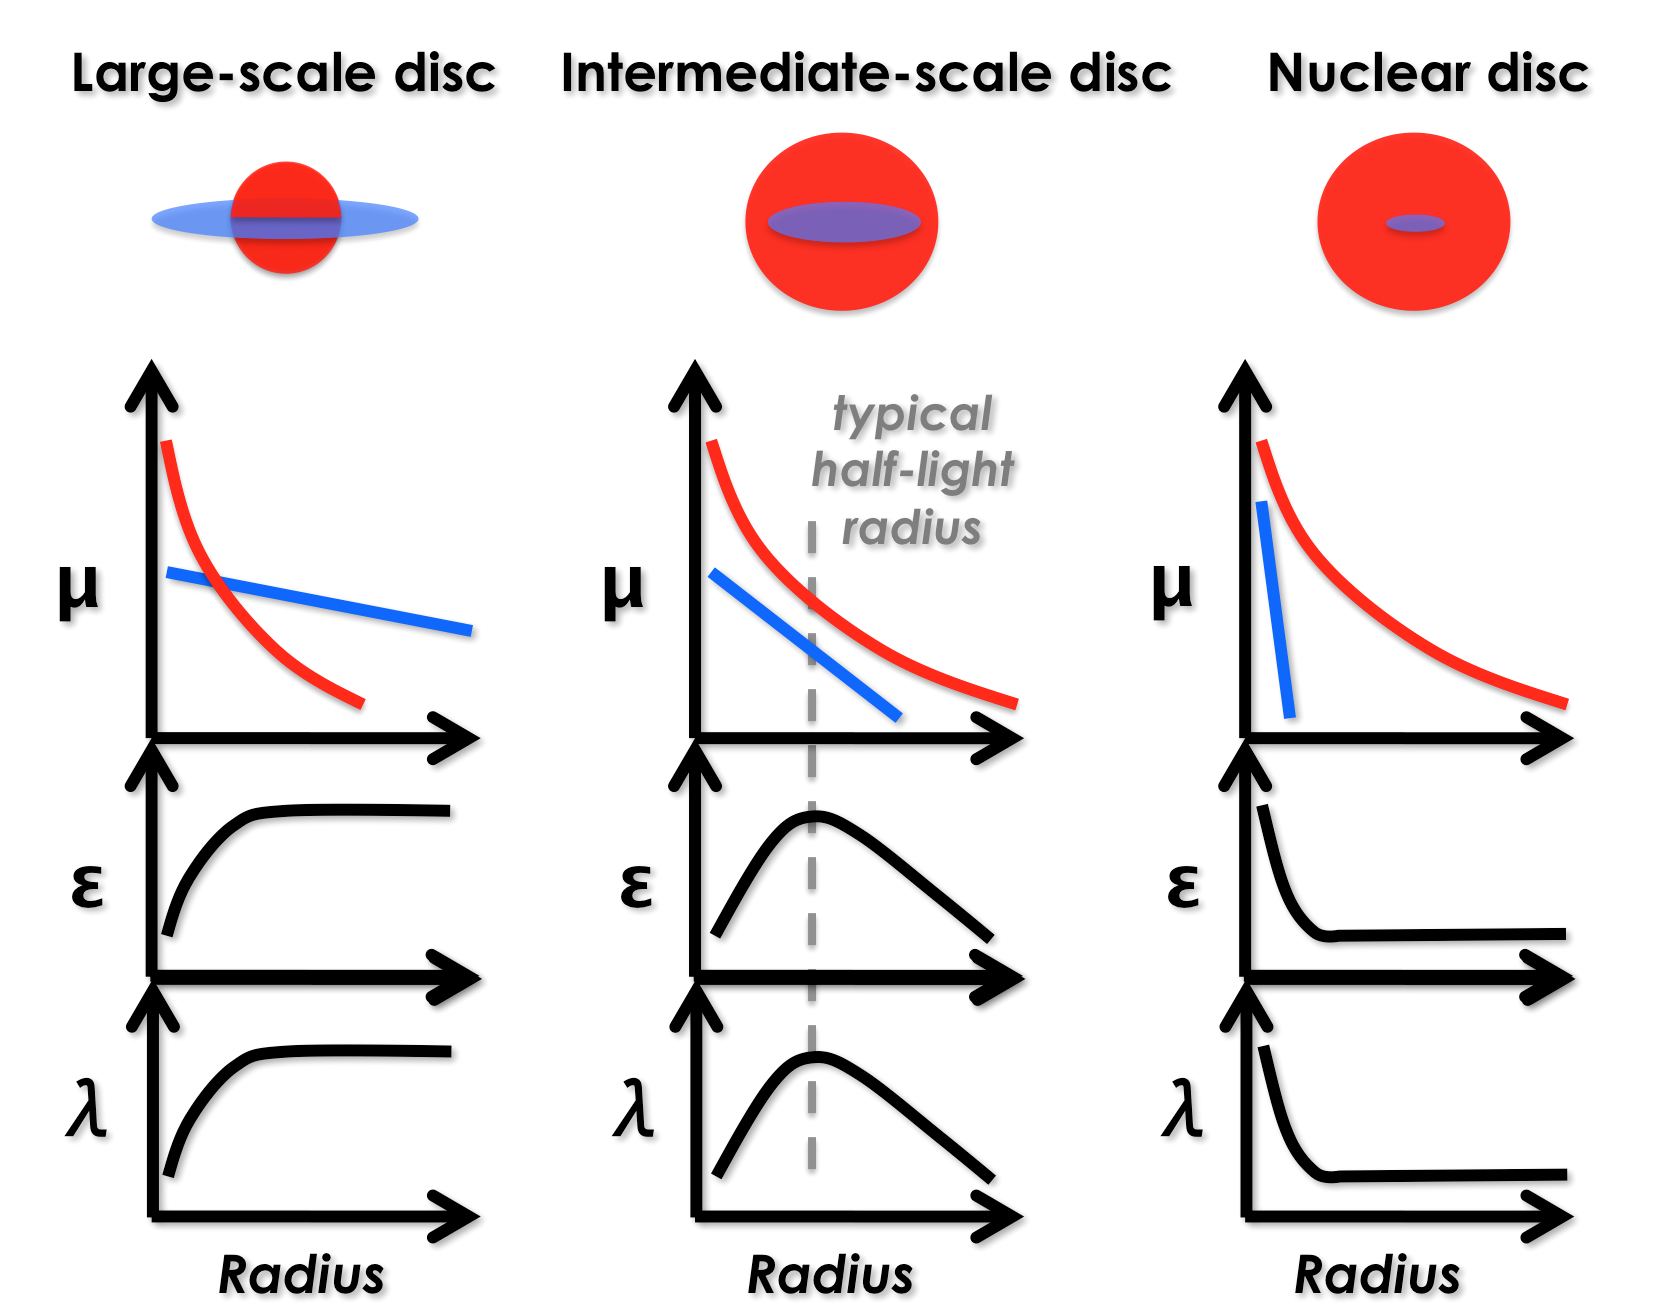
\includegraphics[width=\columnwidth]{images/discmodel.eps}
\caption{Illustration of the spheroid/disc decomposition of the one-dimensional surface brightness profile, $\mu$, 
the ellipticity profile, $\epsilon$, and the specific angular momentum profile, $\lambda$,
for the three prototype early-type galaxy sub-classes. 
In the flux decompositions, the spheroid (or bulge) and the disc are shown with the red and blue color, respectively. 
The left panel shows a lenticular galaxy, composed of a bulge encased in a large-scale disc. 
The right panel displays an elliptical galaxy with (an optional) nuclear stellar disc. 
The middle panel presents an early-type galaxy with an intermediate-sized disc embedded in the spheroid. }
\label{fig:model}
\end{center}
\end{figure}

\section{Galaxies}
\label{sec:gal}
Three examples of early-type galaxies with intermediate-scale discs are NGC 3115, Mrk 1216, and NGC 1271. 
In the following Sections, we present a photometric analysis of these three galaxies, 
and we compare our results with the kinematical analysis (when) available from the literature. 
For the galaxy NGC 3115, we used a $3.6~\rm \mu m$ image obtained with the InfraRed Array Camera (IRAC) 
onboard the \emph{Spitzer Space Telescope}. 
For the galaxies Mrk 1216 and NGC 1271, we used archived Hubble Space Telescope (\emph{HST}) images 
taken with the Wide Field Camera 3 (\emph{WFC3}) and the near-infrared \emph{F160W} filter ($H$-band). 
Our galaxy decomposition technique is extensively described in Savorgnan \& Graham (\emph{submitted}).
Briefly, the galaxy images were background-subtracted, and masks for contaminating sources were created. 
The one-dimensional Point Spread Function (PSF) was characterized for each individual image 
using a Gaussian or a \cite{moffat1969} profile.
We performed an isophotal analysis of the galaxies using the IRAF\footnote{IRAF 
is the Image Reduction and Analysis Facility, distributed by the National Optical Astronomy Observatory, 
which is operated
by the Association of Universities for Research in Astronomy (AURA) 
under cooperative agreement with the National Science Foundation.} task {\tt ellipse}\footnote{isofit...} \citep{taskellipse}. 
The galaxy isphotes were modelled with a series of concentric ellipses, 
allowing the ellipticity, the position angle and the amplitude of the fourth harmonic to vary with radius.  
The decomposition of the surface brightness profiles was performed with software written by G. Savorgnan.
We modelled the light profiles with a combination of PSF-convolved analytic functions, 
using one function per galaxy component. 


\subsection{NGC 3115}
The presence of a disc in NGC 3115 is obvious due to its edge-on orientation (see Figure \ref{fig:n3115}). 
Less obvious is the extent of such disc, if one only relies on a visual inspection of the galaxy image. 
However, the ellipticity profile is consistent with the presence of an intermediate-scale disc. 
Moreover, the kinematics of NGC 3115 disprove the presence of a large scale disc, 
because the galaxy is rapidly rotating only within two effective radii ($\sim 2 \times 50~\rm arcsec$), 
whereas the rotation significantly drops at larger radii \citep{arnold2011n3115}.  
The unsharp mask (Figure \ref{fig:n3115}) of NGC 3115 betrays the presence of a fain edge-on nuclear ring, 
which can also be spotted as a small peak in the ellipticity profile 
(at semimajor-axis lenght $R_{\rm maj} \sim 15~\rm arcsec$).







Two examples of ellicular galaxies are Mrk 1216 and NGC 3115. 
While the presence of a disc in NGC 3115 is obvious due to its edge-on orientation (Figure 3), 
the disc in Mrk 1216 is not immediately apparent from the image 
-- which is partly why many stellar discs have been over-looked to date. 
However the radial light profile and the ellipticity profile betray the presence of a disc in both galaxies. 
The radial light profiles of Mrk 1216 and NGC 3115 extend out to almost four times (4 x 7 arcsec) 
and five times (5 x 50 arcsec) the galaxy half-light radii, respectively. 
The main distribution of light in both of these galaxies is well described with a S\'ersic function22 
for the spheroidal component plus an exponential function for the intermediate-sized disc. 
Moreover, our photometric analysis enables the recovery of an additional nuclear disc in Mrk 1216 
and a nuclear ring in NGC 3115. 
The spheroid/disc decomposition for NGC 3115 is also in excellent agreement with the galaxy's kinematic properties23. 
This comparison cannot be made for Mrk 1216 because no extended kinematic data are available.  
Our models with an intermediate-sized disc embedded within a larger spheroidal component, 
plus an additional nuclear component when one is present, 
match the observed light distribution, and explain both the kinematic maps15 (when available) 
and the ellipticity profiles, of three other ellicular galaxies 
for which a direct measurement of their central supermassive black hole mass is available: 
NGC 1271; NGC 1277; and NGC 1332.  
Past models that ``forcedly'' described these ellicular galaxies with an inner bulge 
encased within a large-scale disc 
typically required the addition of an extended envelope or halo to account for the outer portion of the spheroid. 
Such three-component models (bulge + disc + envelope) reduce the spheroid luminosity by a factor of 2-3, 
and underestimate the size of the spheroid by a factor of 10.

\begin{figure}
\begin{center}
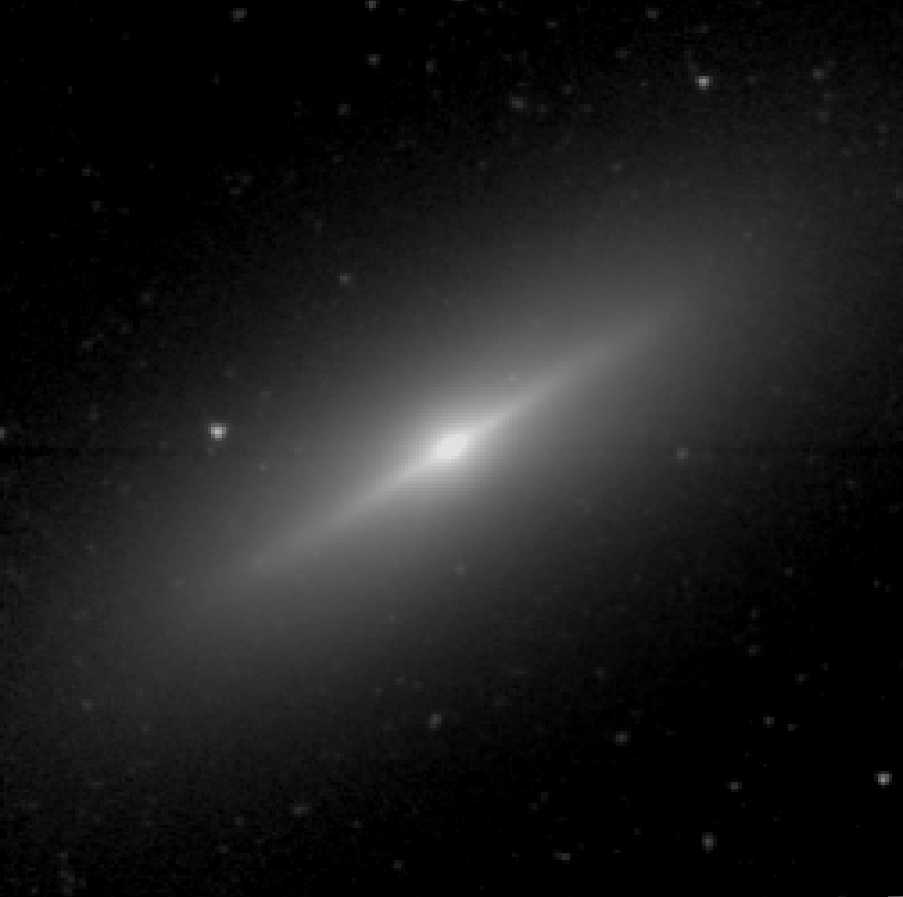
\includegraphics[width=0.49\columnwidth]{images/n3115_image.jpeg}
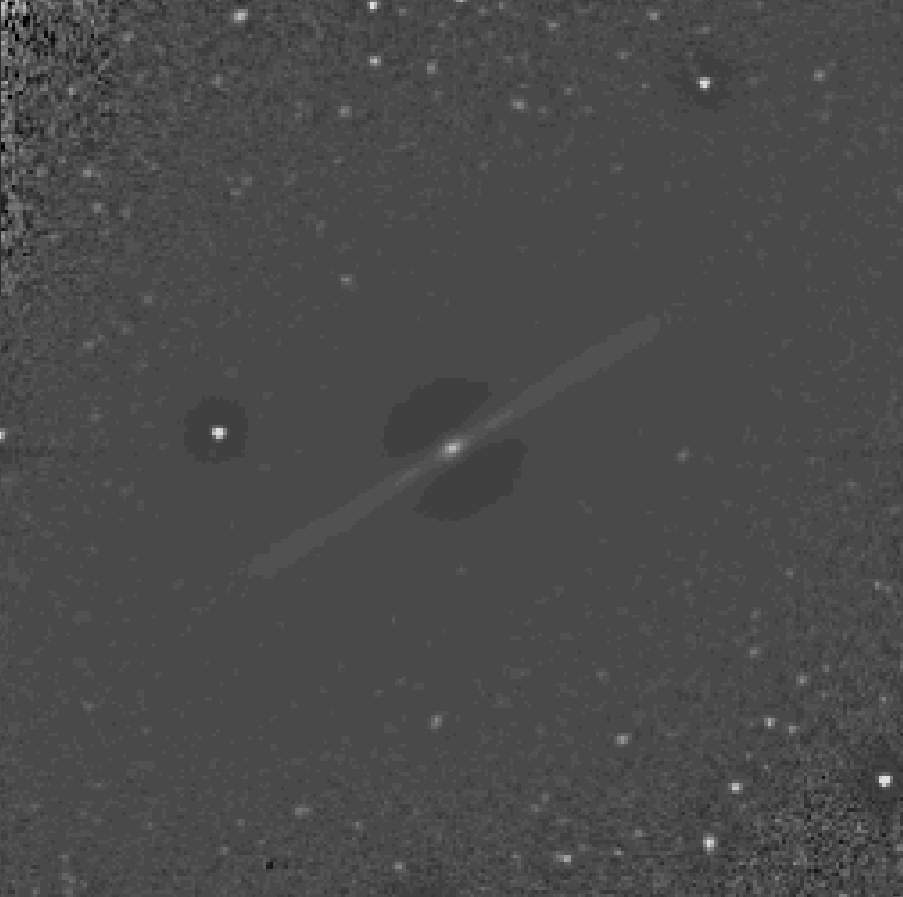
\includegraphics[width=0.49\columnwidth]{images/n3115_unsharp.jpeg} \\
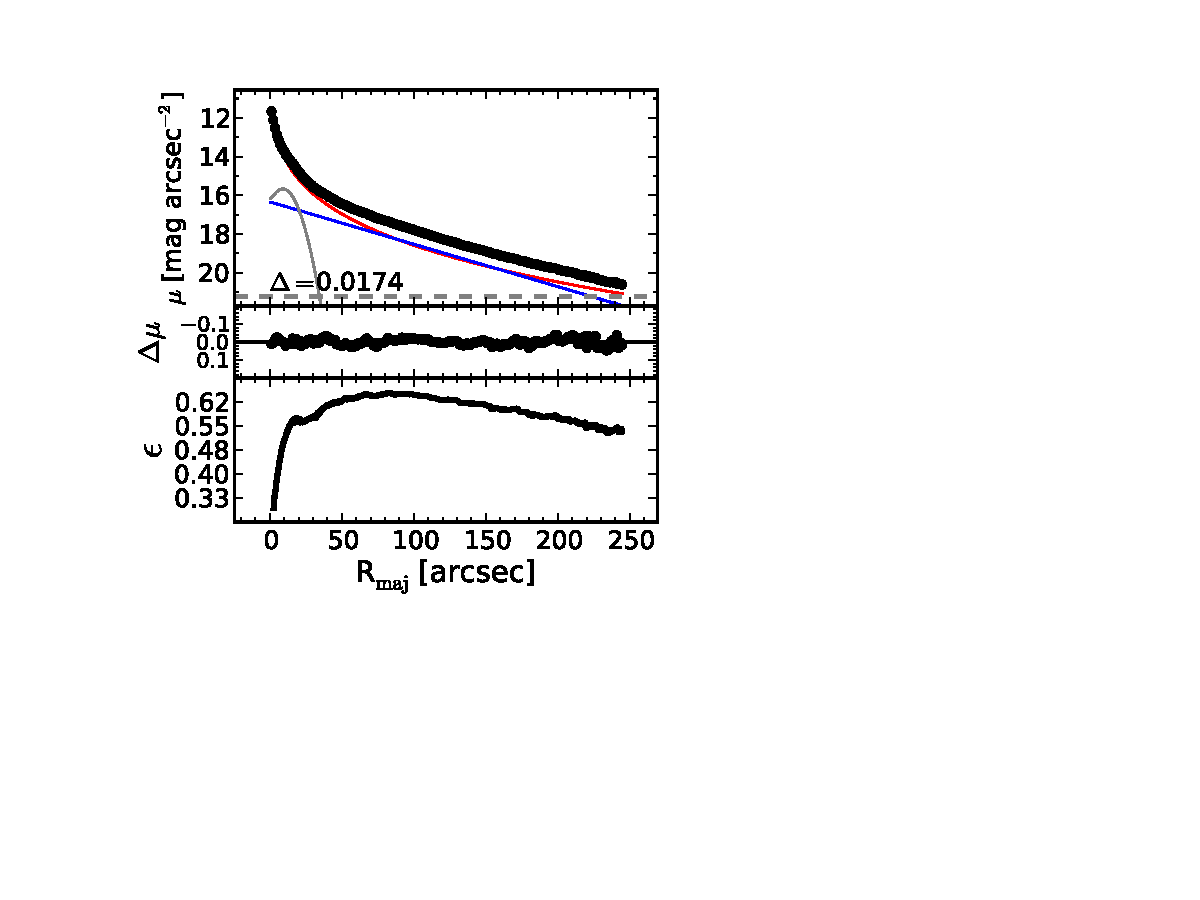
\includegraphics[width=1.05\columnwidth]{images/n3115_decomposition.pdf}
\caption{}
\label{fig:n3115}
\end{center}
\end{figure}

\begin{figure}
\begin{center}
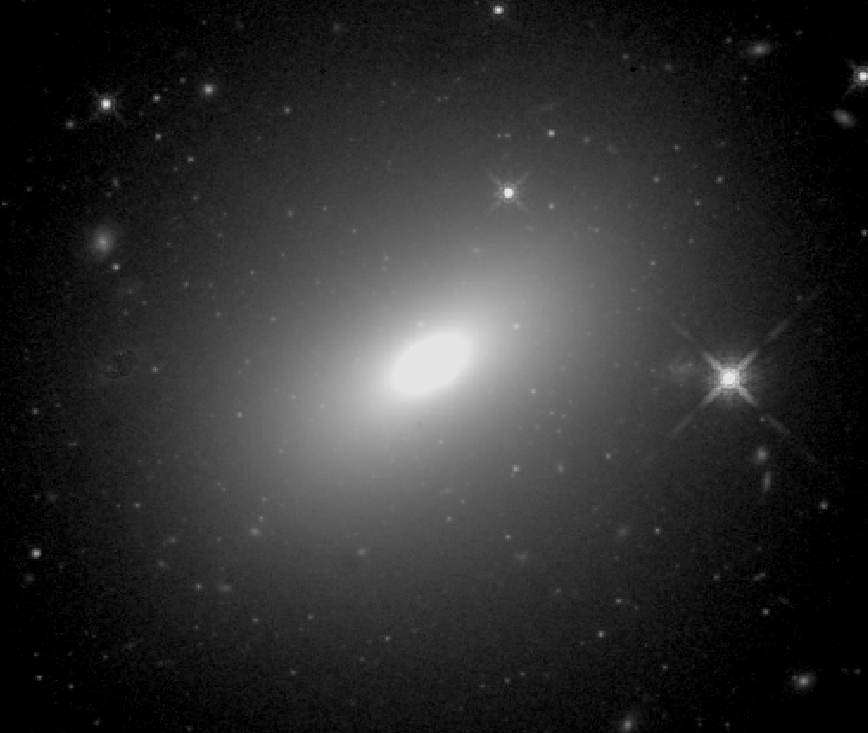
\includegraphics[width=0.49\columnwidth]{images/mrk1216_image.jpeg}
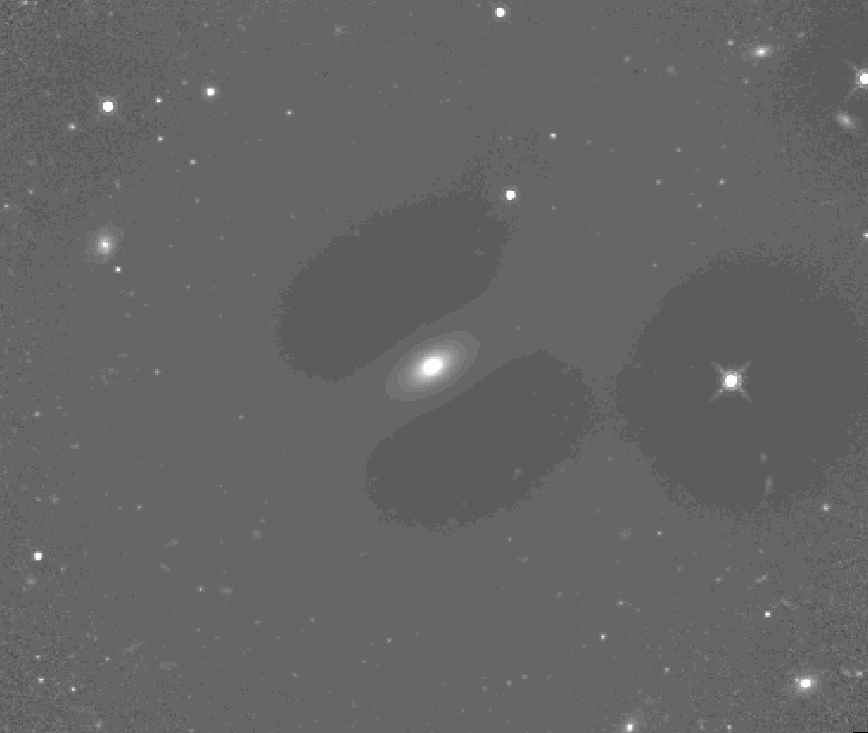
\includegraphics[width=0.49\columnwidth]{images/mrk1216_unsharp.jpeg} \\
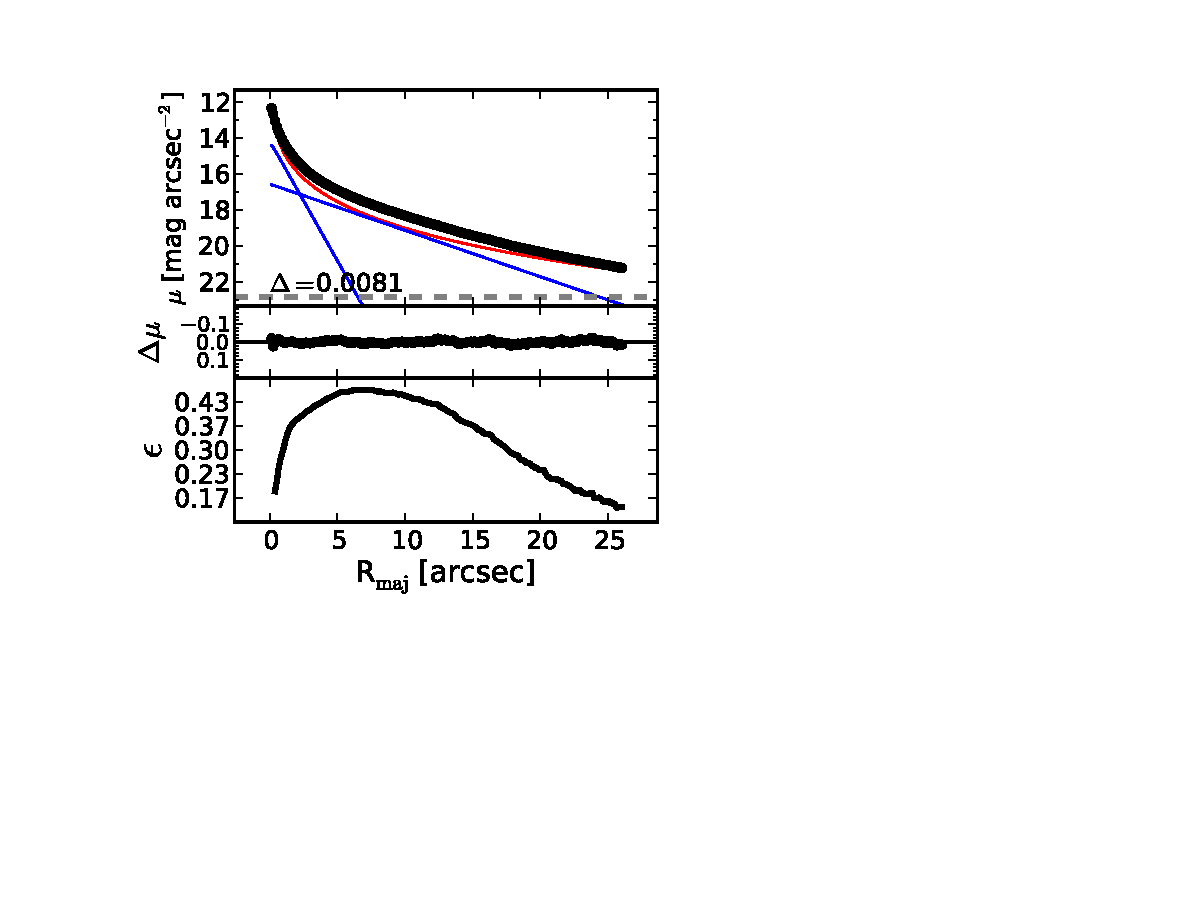
\includegraphics[width=1.05\columnwidth]{images/mrk1216_decomposition.pdf}
\caption{}
\label{fig:m1216}
\end{center}
\end{figure}

\begin{figure}
\begin{center}
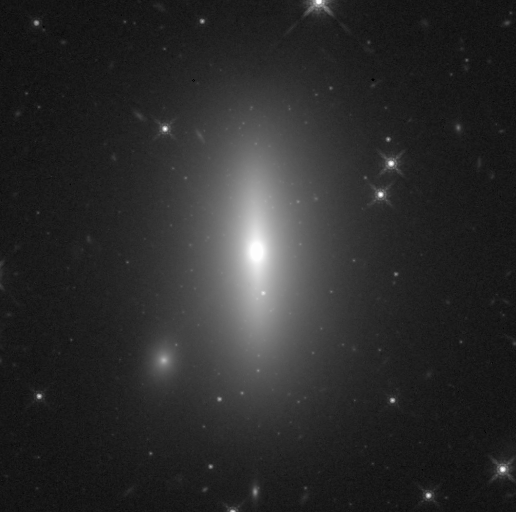
\includegraphics[width=0.49\columnwidth]{images/n1271_image}
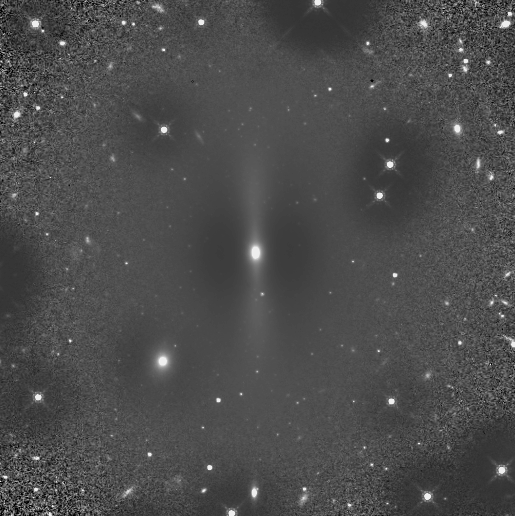
\includegraphics[width=0.49\columnwidth]{images/n1271_unsharp} \\
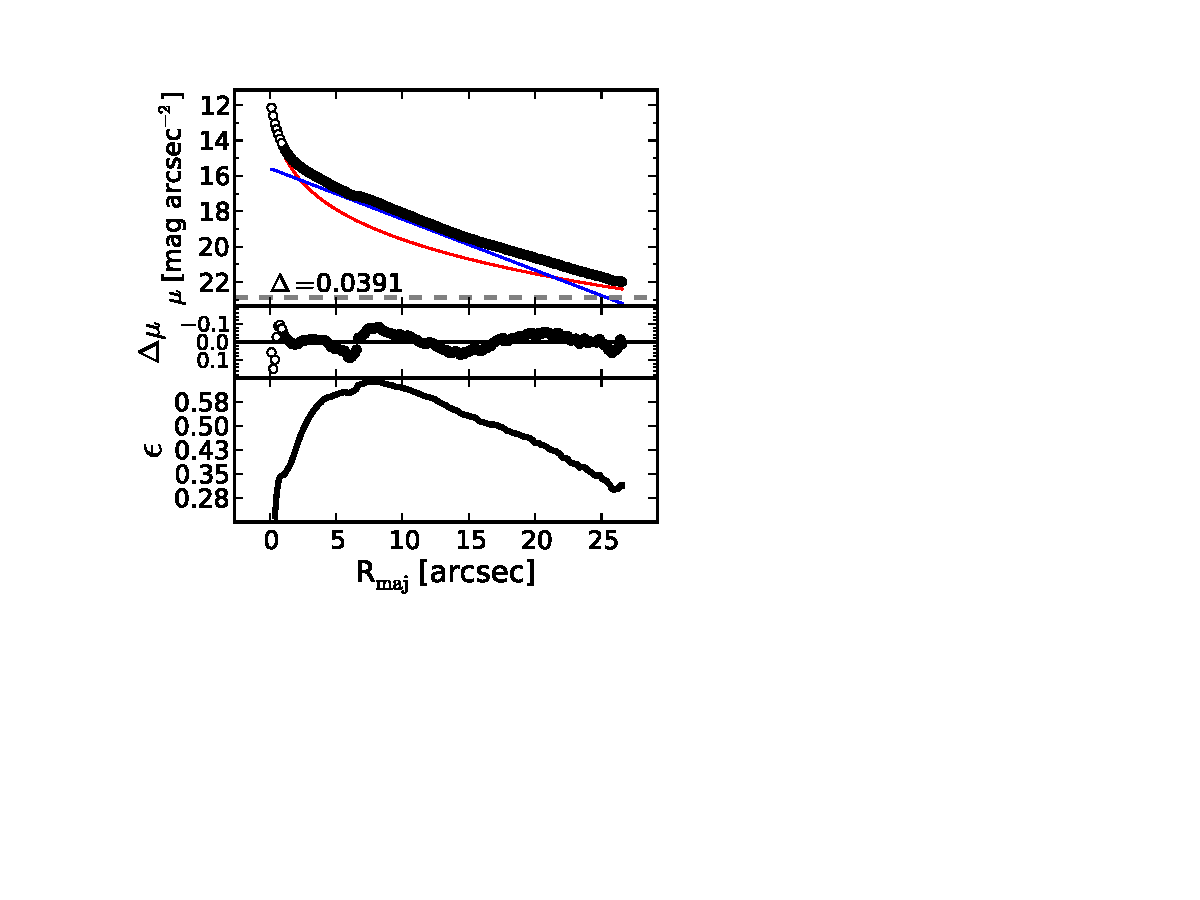
\includegraphics[width=1.05\columnwidth]{images/n1271_decomposition.pdf}
\caption{}
\label{fig:m1216}
\end{center}
\end{figure}



\section{Implications}
\label{sec:impl}

\subsection{mm diagram}
Obviously, having both the black hole mass and the spheroid mass correct is important 
for placing systems in the (black hole mass)-(spheroid stellar mass) diagram. 
For early-type galaxies, the spheroid luminosity and the total galaxy luminosity 
can be used to predict the black hole mass with the same level of accuracy \citep{savorgnan2015}. 
If a galaxy hosts a black hole that is over-massive compared to expectations from the spheroid luminosity, 
but whose mass is normal compared to expectations from the total galaxy luminosity, 
one should wonder whether the spheroid luminosity might have been underestimated 
due to an inaccurate spheroid/disc decomposition. 
Indeed, none of the five ellicular galaxies mentioned here is a noticeable outlier 
in the (black hole mass)-(total galaxy luminosity) diagram \citep{savorgnan2015}. 
For the first time, Figure 4 reveals that when ellicular galaxies are properly modeled, 
they no longer appear as extreme outliers in the (black hole mass)-(spheroid stellar mass) diagram.  

\subsection{compact massive sph}
Acknowledging the correct structure of ellicular galaxies is also important to properly understand their origin. 
According to the current paradigm of cosmological structure evolution, 
the genesis of massive early-type galaxies is characterized by two distinct phases: ''in-situ'' and ''ex-situ''. 
The first phase takes place in a young Universe (within its first 4 billion years), 
when cold gas inflows produced short and intense bursts of star formation that created the cores of galaxies. 
These naked and compact cores, named ''red nuggets''25, have been observed26 at high-redshift with sizes of 1-2 kpc.
In the second phase (last 10 billion years), stellar discs and stellar envelopes 
were accreted around these primordial galaxy cores and assembled the external parts of galaxies on scales of 2-20 kpc. 
Today's Universe is populated by an abundance of compact, massive spheroids27, 
with the same physical properties -- mass and compactness -- as the high-redshift red nuggets. 
Some of these local compact massive spheroids are encased within a large-scale disc, 
that is to say they are the bulges of some lenticular and spiral galaxies. 
Over the last 10 billion years their spheroids have evolved by growing a relatively flat disc -- 
rather than a three-dimensional envelope -- 
which has increased the galaxy size but preserved the bulge compactness. 
The other compact massive spheroids of today's Universe belong to some ellicular galaxies. 
Indeed, Mrk 1216, NGC 1271, NGC 1277, NGC 1332, and NGC 3115 are all local compact ellicular galaxies 
with purely old (>10 billion years) stellar populations. 
These galaxies have undergone the lowest degree of disc growth.
In addition to the observational clues as to the actual physical components in ellicular galaxies, 
one can reason on other grounds as to why these compact galaxies are not comprised of an inner bulge 
plus large-scale disc plus outer envelope5,28,6. If they were such three-component systems, 
then one would have two possibilities. 
The first possibility is that these galaxies were already fully assembled 10 billion years ago; 
this would explain their old stellar populations, 
but it would also imply that their discs and envelopes had already formed during the first 4 billion years of the Universe, 
in disagreement with the current cosmological picture. 
The second possibility is that only their inner bulges (with sizes of 0.1-0.2 kpc, 
according to past decompositions) originated in the first 4 billion years 
and they subsequently accreted a substantial disc and envelope. 
If this was correct, then we would observe high-redshift, star-like, naked bulges with stellar masses 
within a factor of a few times the currently observed red nuggets but sizes which are 10 times smaller. 
However, a dramatically different expectation is reached 
if one considers these galaxies as spheroid-dominated systems with an intermediate-scale disc; 
in this case, both the galaxy size and the spheroid size are compact (1-2 kpc). 
This implies that, among the local descendants of the high-redshift red nuggets, 
the compact ellicular galaxies have undergone the lowest degree of disc growth. 
That is, the bulk of a compact ellicular galaxy quickly assembled ''in-situ'' in a very young Universe 
and experienced very little evolution over the last 10 billion years.

\begin{figure}
\begin{center}
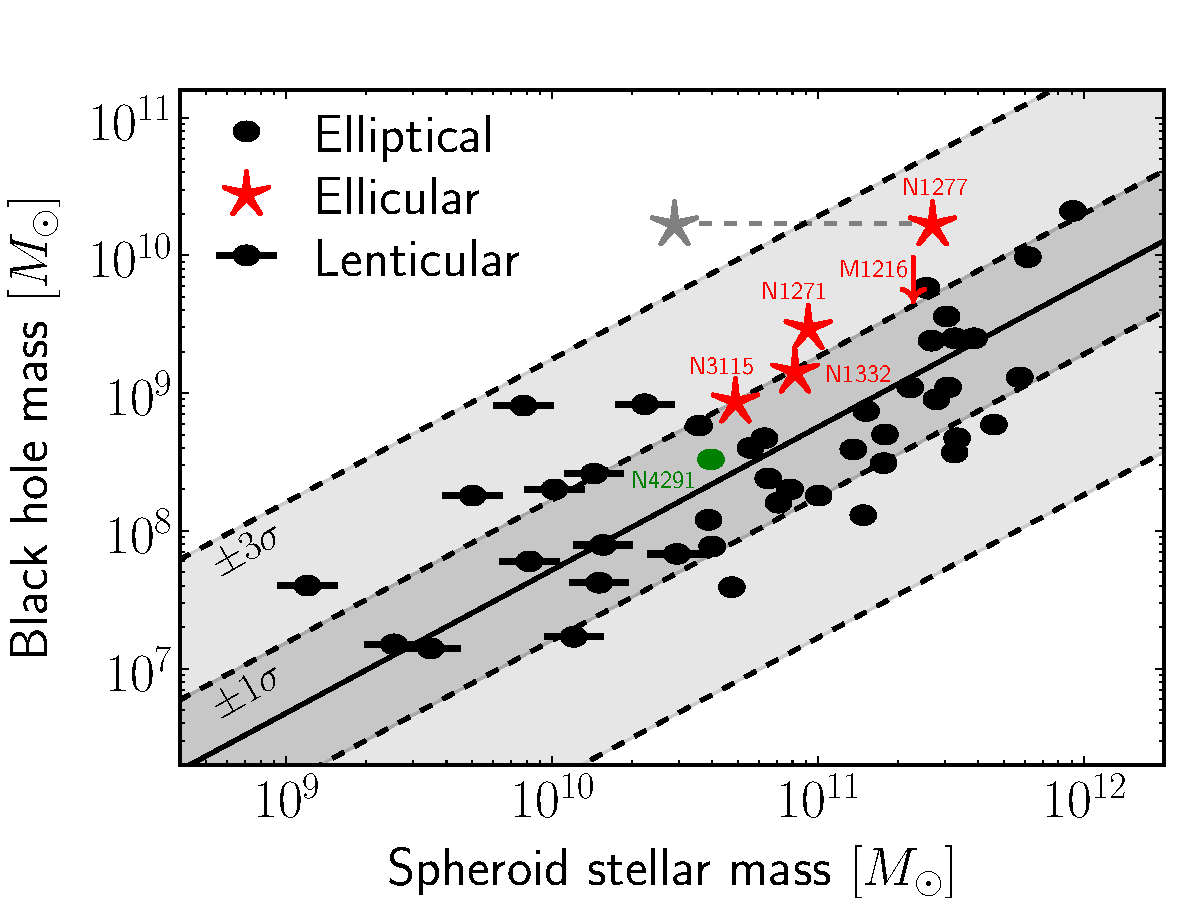
\includegraphics[width=\columnwidth]{images/mm.pdf}
\caption{Early-type galaxies: black hole mass plotted against spheroid stellar mass for 42 galaxies (black) plus the galaxies Mrk 1216, NGC 1271, NGC 1277, NGC 1332, NGC 3115, and NGC 4291. The black solid line is the bisector linear regression for early-type galaxies24. The dashed lines mark the 1sigma and 3sigma deviations, where sigma (0.51 dex) is the total rms scatter about the correlation in the black hole mass direction. The red color is used for five ellicular galaxies, (Mrk 1216, for which only an upper limit on its black hole mass has been reported) [4], NGC 1271 [6], NGC 1277 [5, 4], NGC 1332 [7], and NGC 4291 [29]), that were claimed to be extreme outliers in this diagram. All reside within a 3sigma deviation from the correlation when using their correct spheroid mass. For NGC 1277, we show the previously reported spheroid stellar mass [5] in gray.}
\label{fig:mm}
\end{center}
\end{figure}

%\begin{figure}[h]
%\begin{center}
%\includegraphics[width=\columnwidth]{images/}
%\caption{}
%\label{fig:}
%\end{center}
%\end{figure}


\section{Acknowledgments}
%GS warmly thanks Luca Cortese, Elisabete Lima Da Cunha, Duncan Forbes and Gonzalo Diaz for useful discussion. \\
% referee thank you!!
This research was supported by Australian Research Council funding through grants
DP110103509 and FT110100263.
%This work is based on observations made with the IRAC instrument \citep{fazio2004IRAC} 
%on-board the Spitzer Space Telescope, 
%which is operated by the Jet Propulsion Laboratory, 
%California Institute of Technology under a contract with NASA.
%This research has made use of the GOLDMine database \citep{goldmine} and the NASA/IPAC Extragalactic Database (NED) 
%which is operated by the Jet Propulsion Laboratory, California Institute of Technology, 
%under contract with the National Aeronautics and Space Administration. 

\bibliography{/Users/gsavorgnan/galaxy_vivisection/papers/SMBHbibliography}


\label{lastpage}

\clearpage


\end{document}
